\documentclass{article}
\usepackage{caption}
\usepackage{subcaption}
\usepackage{graphicx}
\usepackage{tikz}
\usepackage{tikzsymbols}
\usetikzlibrary{calc,patterns,shapes.geometric}
\usepackage{float}
\usepackage{pdflscape}
\usepackage{geometry}
\geometry{a4paper, landscape, margin=1cm}

\def\centerarc[#1](#2)(#3:#4:#5){\draw[#1] ($(#2)+({#5*cos(#3)},{#5*sin(#3)})$) arc (#3:#4:#5);}

\pagestyle{empty}
\begin{document}
	\centering
	\begin{figure}[H]
			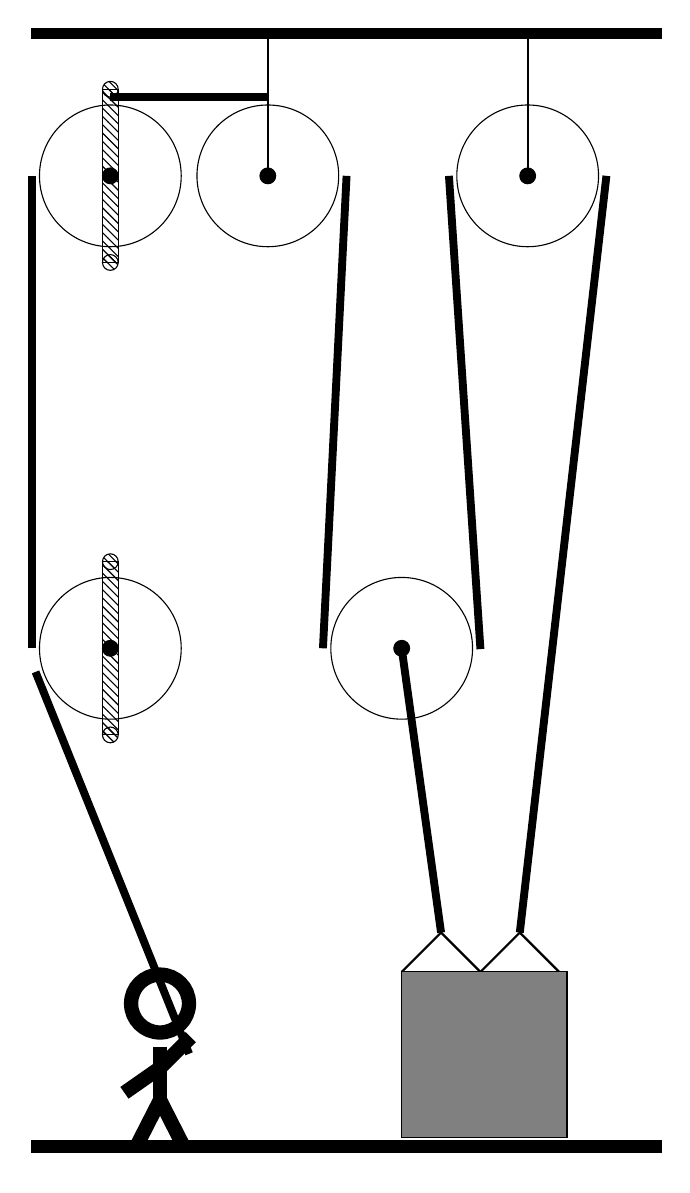
\begin{tikzpicture}
				%%%%% START %%%%%
				\def\a{11}
				\def\radlg{\radrp-0.1}
				\def\radrp{1.0}
				\def\radsm{0.1}
				\def\xone{1}
				\def\yone{\a-1.75}
				\def\xtwo{\xone+3.3}
				\def\ytwo{\a-1.75}
				\def\xthree{\xone+1.7}
				\def\ythree{\a-7.75}
				\def\xh{3.2}
				\def\hlentwo{\yone+3.14}
				\def\hlen{\yone+3.14}
				\def\width{1mm}
				\def\ywallone{\yone}
				\def\xwallone{\xone-2}
				\def\ywalltwo{\ythree}
				\def\xwalltwo{\xone-2}
				
				\draw[fill=black] (-2,\a) rectangle (6,\a+0.125);

				\draw (\xone,\yone) circle (\radlg);
				\draw[fill=black] (\xone,\yone) circle (\radsm);
				\draw[thick] (\xone,\yone) -- (\xone,\a);

				\draw (\xtwo,\ytwo) circle (\radlg);
				\draw[fill=black] (\xtwo,\ytwo) circle (\radsm);
				\draw[thick] (\xtwo,\ytwo) -- (\xtwo,\a);

				\draw (\xthree,\ythree) circle (\radlg);
				\draw[fill=black] (\xthree,\ythree) circle (\radsm);


				\draw[thick]  (\xh-0.5,\ytwo-\hlentwo-0.5) -- (\xh,\ytwo-\hlentwo) -- (\xh+0.5,\ytwo-\hlentwo-0.5);
				\draw[thick]  (\xh+0.5,\yone-\hlen-0.5) -- (\xh+1,\yone-\hlen) -- (\xh+1.5,\yone-\hlen-0.5);
				\draw[fill=black!50] (\xh-0.5,\yone-\hlen-0.5) rectangle (\xh+1.6,\yone-\hlen-0.5-2.1);
				
				%first extra polly
				\draw[pattern=north west lines, pattern color=black] (\xwallone-0.1,\ywallone+\radrp+0.1) rectangle (\xwallone+0.1,\ywallone-\radrp-0.1); 
				\draw[pattern=north west lines, pattern color=black] (\xwallone,\ywallone+\radrp+0.1) circle (\radsm);
				\draw[pattern=north west lines, pattern color=black] (\xwallone,\ywallone-\radrp-0.1) circle (\radsm);
				
				\draw (\xwallone,\ywallone) circle (\radlg);
				\draw[fill=black] (\xwallone,\ywallone) circle (\radsm);
				
				% second extra
				\draw[pattern=north west lines, pattern color=black] (\xwalltwo-0.1,\ywalltwo+\radrp+0.1) rectangle (\xwalltwo+0.1,\ywalltwo-\radrp-0.1); 
				\draw[pattern=north west lines, pattern color=black] (\xwalltwo,\ywalltwo+\radrp+0.1) circle (\radsm);
				\draw[pattern=north west lines, pattern color=black] (\xwalltwo,\ywalltwo-\radrp-0.1) circle (\radsm);
				
				\draw (\xwalltwo,\ywalltwo) circle (\radlg);
				\draw[fill=black] (\xwalltwo,\ywalltwo) circle (\radsm);
				
				
				
				\draw[line width=\width](\xone-\radrp,-1.9) -- 	(\xwalltwo-\radrp*0.95, \ywalltwo-\radrp*0.3);
				\centerarc[line width=\width](\xwalltwo,\ywalltwo)(180:210:\radrp);
				\draw[line width=\width](\xwalltwo-\radrp, \ywalltwo) -- (\xwallone-\radrp, \ywallone);
				\centerarc[line width=\width](\xwallone,\ywallone)(90:180:\radrp);
				
				\draw[line width=\width](\xwallone, \ywallone+\radrp) -- (\xone,\yone+\radrp);
				\centerarc[line width=\width](\xone,\yone)(0:90:\radrp);
				\draw[line width=\width](\xone+\radrp,\yone) -- (\xthree-\radrp,\ythree);
				\centerarc[line width=\width](\xthree,\ythree)(180:370:\radrp);
				\draw[line width=\width] (\xthree+\radrp,\ythree-0.01) -- (\xtwo-\radrp,\ytwo);
				\centerarc[line width=\width](\xtwo,\ytwo)(0:180:\radrp);
				\draw[line width=\width](\xh+1,\yone-\hlen) -- (\xtwo+\radrp,\ytwo);
				\draw[line width=\width] (\xh,\yone-\hlen) -- (\xthree,\ythree);

				\node at (-0.4,-2) {\Strichmaxerl[10][35][45]};
						
				\draw[fill=black] (-2,-3) rectangle (6,-3.15);
				%%%%% START %%%%%
			\end{tikzpicture}
	\end{figure}

\end{document}